\documentclass[
  aps,            % American Physical Society style
  prc,            % Physical Review C
  reprint,        % two-column published format; use "preprint" for the one-column manuscript style
  superscriptaddress,
  floatfix,
  nofootinbib
]{revtex4-2}

% ---------------------------------------------------------------------------
%  Paper II of two: resolution refinement + rodeo algorithm on the pairing
%  Hamiltonian supplemented by a seniority-breaking particle-hole interaction.
%  Built from the Jupyter notebook ResolutionRefPairing.ipynb (sections
%  EXT:PH, EXT:BOUND and the particle-hole rows of EXT:BASELINES).
%  Paper I (pure pairing model) is paper/eigenq_pairing.tex, cited as
%  \cite{PairingCompanion}.  RevTeX 4-2 / APS style.
% ---------------------------------------------------------------------------

\usepackage{amsmath,amssymb}
\usepackage{physics}
\usepackage{graphicx}
\usepackage{hyperref}

\newcommand{\Hlow}{H_{\mathrm{low}}}
\newcommand{\Hhigh}{H_{\mathrm{high}}}
\newcommand{\Eobj}{E_{\mathrm{obj}}}
\newcommand{\Vph}{V_{\mathrm{ph}}}

\begin{document}

\title{Resolution refinement and the rodeo algorithm beyond seniority:
eigenstate preparation for the pairing Hamiltonian with a particle-hole
interaction}

\author{Scott Bogner}
\affiliation{Facility for Rare Isotope Beams and Department of Physics and Astronomy, Michigan State University, East Lansing, MI 48824, USA}
\author{Cecilie Glittum}
\affiliation{Department of Physics, University of Oslo, N-0316 Oslo, Norway}
\author{Heiko Hergert}
\affiliation{Facility for Rare Isotope Beams and Department of Physics and Astronomy, Michigan State University, East Lansing, MI 48824, USA}
\author{Morten Hjorth-Jensen}
\email{mhjensen@uio.no}
\affiliation{Department of Physics, University of Oslo, N-0316 Oslo, Norway}
\author{Gunnar Lange}
\affiliation{Department of Physics, University of Oslo, N-0316 Oslo, Norway}
\author{Ryan LaRose}
\affiliation{Department of Computational Mathematics, Science and Engineering and Facility for Rare Isotope Beams, Michigan State University, East Lansing, MI 48824, USA}
\author{Dean Lee}
\affiliation{Facility for Rare Isotope Beams and Department of Physics and Astronomy, Michigan State University, East Lansing, MI 48824, USA}
\author{Francesco Pietro Massel}
\affiliation{Department of Science and Industry Systems, University of South-Eastern Norway, N-3616 Kongsberg, Norway}
\affiliation{Department of Physics, University of Oslo, N-0316 Oslo, Norway}
\author{Jean Paul Sadia}
\affiliation{Department of Computational Mathematics, Science, and Engineering, Michigan State University, East Lansing, MI 48823, USA}
\affiliation{Center for Quantum Computing, Science, and Engineering, Michigan State University, East Lansing, MI 48823, USA}
\date{\today}

\begin{abstract}
The constant-pairing Hamiltonian conserves seniority, so its ground state
lives in the seniority-zero subspace, the one-particle--one-hole channel is
closed, and a one-qubit-per-pair encoding is available --- properties that
make it a convenient but unusually well-behaved testbed for quantum
eigenstate preparation.  We remove this simplification by adding to the
pairing force a seniority-breaking particle-hole interaction of strength $f$,
which carries the one-particle--one-hole and pair-breaking channels of
realistic two-body interactions, and we repeat on the resulting Hamiltonian
the assessment of a companion paper: resolution refinement --- the adiabatic
transport of an eigenstate from a coarse to a fine single-particle basis
along a shift-controlled, gapped path --- followed by the rodeo algorithm as
a projective energy filter, compared against the same filter applied to a
full-space unitary coupled-cluster (UCCSD) state, with the ground-state
infidelity as the common observable and a two-qubit gate budget per accepted
preparation.  For four particles on four levels (eight system qubits) at
$f=0.05$, $0.2$ and $0.5$ the structure, operating point and convergence of
the pipeline are unchanged: the path gap is still set by the energy shift,
the refinement time grows from $16$ to $32$ only because the prolonged
starting state loses overlap, and is governed by the renormalized pairing
strength $g+2f$; the filter converges geometrically to an infidelity of
$4.5\times10^{-5}$ after ten cycles at the strongest pair breaking.  The
price of the more realistic interaction appears where it should, in the
Pauli-string content of the Hamiltonian ($61\to325$ strings on eight
qubits, maximal weight $4\to8$) and hence in the depth of a Trotter step
($296\to2728$ CNOTs), which raises the budget per accepted preparation from
$7\times10^{4}$ to $6$--$8\times10^{5}$ CNOTs.  The single-reference UCCSD
ansatz, exact for the pairing force at the coarse resolution and accurate to
$1.8\times10^{-4}$ in infidelity at the fine one, degrades twentyfold across
the scan as the ground state acquires seniority-two weight, yet filtering it
still reaches a lower infidelity than the refined input at a factor two to
three lower cost.  The sufficient adiabatic-time and Trotter-step conditions
available for such paths are evaluated and shown to be insensitive to the
pair breaking in the time and sensitive to it in the step count.
\end{abstract}

\maketitle

% ===========================================================================
\section{Introduction}
% ===========================================================================
Schematic nuclear Hamiltonians --- pairing, Lipkin and small shell-model
interactions --- are the standard proving ground for quantum algorithms in
nuclear structure~\cite{Beck2023,Bauer2023,LeeReview2023,Ovrum2007,Hlatshwayo2022,Stetcu2022,PerezObiol2023,Jiang2023,Zhang2024,Lacroix2023},
and the constant-pairing model in particular, integrable by the Richardson
ansatz~\cite{Richardson1963,RichardsonSherman1964,Dukelsky2004}, has become
the model of choice: the programme of Lacroix and collaborators on symmetry
breaking and restoration~\cite{Lacroix2020,RuizGuzman2022,RuizGuzman2023,RuizGuzman2024,Lacroix2023EPJA,Ayral2023},
on ADAPT-VQE with symmetry-conserving and symmetry-breaking
pools~\cite{Zhang2024,Zhang2025} and on Green's functions of small
superfluid systems~\cite{AychetClaisse2026} is built largely on it, and so is
the companion paper to the present work~\cite{PairingCompanion}, in which we
implemented and assessed, stage by stage against exact results, a pipeline
for eigenstate preparation that combines \emph{resolution
refinement}~\cite{Bogner2026} --- the adiabatic transport of a
coarse-resolution eigenstate, lifted by a prolongation operator into a finer
single-particle basis, along a shift-controlled gapped path --- with the
\emph{rodeo algorithm}~\cite{Choi2021,Qian2024} as a projective energy
filter.  The finding of that assessment was, on the question that decides
whether the refinement stage earns its gates, negative: compared on the same
observable, the ground-state infidelity, and with the same Trotterized
filter, refinement followed by the rodeo algorithm does not outperform the
filter applied to a full-space unitary coupled-cluster (UCCSD) state at any
size that can be validated exactly; what the refinement offers in exchange
is freedom from classical optimization and training measurements.

The pairing Hamiltonian is, for the purpose of testing methods, almost too
well behaved.  The pairing force moves complete time-reversed pairs and does
nothing else: it conserves the seniority (the number of unpaired particles),
the $N=4$ ground state on $k$ levels lives in a $\binom{k}{2}$-dimensional
seniority-zero space, and an entire class of excitations is absent --- there
is no matrix element between the reference determinant and any
one-particle--one-hole state.  The model is by no means outside the reach of
mean-field-based methods --- the Richardson model has long served as a
testing ground for particle-particle RPA and its self-consistent and
renormalized variants~\cite{Hirsch2002,Dang2006} and for the quasiparticle
RPA~\cite{RingSchuck} --- but the particle-hole channel on which
Tamm--Dancoff and particle-hole RPA are built is simply closed in it.
Realistic nuclear and electronic Hamiltonians do have that channel.  Two
consequences follow for quantum state preparation.  A single-reference
variational ansatz is unusually accurate for the pure pairing force, because
the singles amplitudes vanish identically and the ansatz is effectively a
doubles theory; and the compact one-qubit-per-pair encoding used in much of
the pairing-model literature~\cite{Lacroix2020,AychetClaisse2026} is
available only because the seniority is conserved.  Neither property
survives a seniority-breaking interaction, and an assessment carried out
on the pairing model alone is therefore silent on precisely the regime ---
a degrading variational input, a full fermionic register --- in which an
optimizer-free preparation such as refinement might be expected to pay off.

In this paper we open the particle-hole channel.  Following Chapter~4 of
Ref.~\cite{MHJbook} we add to the pairing force a single extra term, a
particle-hole interaction $\Vph$ of strength $f$ that contains, besides a
renormalization of the pairing strength, one-particle--one-hole excitations
of seniority two and seniority-two two-particle--two-hole excitations, and
we keep everything else --- the level scheme, the particle number $N=4$, the
resolutions $k=2,3,4$, the $2k$-qubit Jordan--Wigner register, and every
stage and setting of the pipeline --- exactly as in
Ref.~\cite{PairingCompanion}, so that each change in the results can be
attributed to the interaction alone.  The strengths $f=0.05$, $0.2$ and
$0.5$ at $g=1$ are those of Ref.~\cite{MHJbook}, whose tables every exact
number below reproduces.  We ask five questions: whether the pipeline runs
unchanged on a Hamiltonian with a denser, seniority-mixed spectrum; how the
refinement time and the path gap respond to the pair breaking; how the rodeo
filter behaves when its energy scan sees a denser spectrum; what the extra
channels cost at the circuit level, in Pauli strings, Trotter depth and
two-qubit gates per accepted preparation; and whether the verdict on the
refinement stage against the filtered UCCSD input changes once the
variational input itself starts to degrade.

The paper is organized as follows.  Section~\ref{sec:model} defines the
Hamiltonian and its qubit encoding.  Section~\ref{sec:pipeline} recalls the
stages of the pipeline, the cost accounting and the pure-pairing reference
numbers of Ref.~\cite{PairingCompanion} that the results are measured
against.  Section~\ref{sec:results} presents the exact and variational
references, the refinement, the sufficient adiabatic conditions and the
rodeo filtering with the particle-hole term, and Sec.~\ref{sec:circuits}
the circuit-level budget.  Section~\ref{sec:discussion} discusses the
findings, the relation to the pairing-model literature, the hardware
requirements and the extensions that follow.

% ===========================================================================
\section{The pairing model with a particle-hole interaction}
\label{sec:model}
% ===========================================================================
The constant-pairing Hamiltonian of Ref.~\cite{PairingCompanion} is
\begin{widetext}
\begin{equation}
  H_{\rm pair}=\delta\sum_{p=0}^{k-1} p\sum_{\sigma=\uparrow\downarrow} n_{p\sigma}
   -\frac{g}{2}\sum_{p,q=0}^{k-1} a^\dagger_{p\uparrow}a^\dagger_{p\downarrow}
     a_{q\downarrow}a_{q\uparrow},
  \label{eq:H}
\end{equation}
\end{widetext}
with $k$ doubly degenerate single-particle levels of spacing $\delta$ (set to
$\delta=1$) and a pairing strength $g$; level $p$ and spin $\sigma$ are mapped
to qubit $2p+\sigma$, so a $k$-level problem uses $2k$ qubits, and the
fermionic operators are encoded through the Jordan--Wigner transformation.
``Basis refinement'' means increasing $k$ at fixed $N$.  To this we add,
following Chapter~4 of Ref.~\cite{MHJbook}, the particle-hole interaction
\begin{equation}
  \Vph=-\frac{f}{2}\sum_{p,q,r=0}^{k-1}\Big(
    a^\dagger_{p\uparrow}a^\dagger_{p\downarrow}a_{q\downarrow}a_{r\uparrow}
    +{\rm h.c.}\Big),
  \label{eq:Vph}
\end{equation}
and study $H=H_{\rm pair}+\Vph$ at $g=1$ and $f=0.05$, $0.2$, $0.5$, with
$f=0$ the pure pairing model as the reference.

The triple sum contains three distinct processes.  The $q=r$ pieces are the
pairing term again and merely renormalize $g\to g+2f$; the $q=p\neq r$ pieces
carry a \emph{single} particle from one level to another, a $1p$--$1h$
excitation of seniority two; and the pieces with $p,q,r$ all different remove
two unpaired particles and deposit a pair elsewhere, a seniority-two $2p$--$2h$
excitation.  $\Vph$ still conserves $N_\uparrow$ and $N_\downarrow$
separately, so $S_z$ remains a good quantum number, but the seniority does
not: at $k=4$ the $S_z=0$ sector has $36$ determinants instead of the six pair
configurations, and the compact one-qubit-per-pair encoding of the pairing
model~\cite{Lacroix2020,AychetClaisse2026} is no longer available.  We keep
the $2k$-qubit Jordan--Wigner register; it is the convenient general choice,
not the only one --- the conserved particle number and $S_z$ still permit
compressed encodings of the $36$-dimensional block --- but it is the register
on which the gate counts below are meaningful, and it is the register on
which the stages of the pipeline were written.  Acting once on the reference
determinant at $k=4$, the Hamiltonian now reaches eight $1p$--$1h$ and eight
seniority-two $2p$--$2h$ determinants with matrix elements $\pm f/2$, in
addition to the four seniority-zero $2p$--$2h$ states whose coupling grows
from $g/2$ to $(g+2f)/2$.  Two consequences matter for the pipeline.  First,
the filled determinant is no longer a stationary Hartree--Fock solution: its
one-particle--one-hole matrix elements $\mel{\Phi_i^a}{H}{\Phi_0}=\pm f/2$ do
not vanish (Brillouin's theorem holds for the self-consistent determinant,
which we have not re-optimized), so the UCCSD \emph{singles}, identically zero
for the pairing force, switch on and absorb part of what an optimized
reference would describe as mean-field relaxation rather than correlation.
Second, the reference energy becomes $E_{\rm ref}=2-g-2f$, and the quantity
we call correlation energy below is measured from this unrelaxed reference.

Table~\ref{tab:pauli} lists the Pauli-string content of $H$ on $2k$ qubits.
The particle-hole term multiplies the number of strings by a factor that
grows with the resolution ($1.8$, $3.5$ and $5.3$ at $k=2,3,4$; $61\to325$ at
$k=4$) and raises the largest Pauli weight from four to $2k$ ($8$ at $k=4$),
because a $1p$--$1h$ string drags a Jordan--Wigner parity chain across the
register.  This table is the origin of every increase in circuit depth
reported in Sec.~\ref{sec:circuits}.

\begin{table}[t]
\caption{\label{tab:pauli}Pauli-string content of the Hamiltonian on $2k$
qubits: number of strings and largest Pauli weight, for the pairing model and
for the pairing model with the particle-hole term ($f\neq0$; the counts do not
depend on the value of $f$).  The $k=2,3$ rows agree with Ref.~\cite{MHJbook}.}
\footnotesize
\begin{ruledtabular}
\begin{tabular}{cccc}
$k$ & qubits & pairing & pairing $+$ $\Vph$\\
\colrule
2 & 4 & $15$ (weight $4$) & $27$ (weight $4$)\\
3 & 6 & $34$ (weight $4$) & $118$ (weight $6$)\\
4 & 8 & $61$ (weight $4$) & $325$ (weight $8$)\\
\end{tabular}
\end{ruledtabular}
\end{table}

% ===========================================================================
\section{The pipeline, its cost accounting, and the pure-pairing reference}
\label{sec:pipeline}
% ===========================================================================
We recall the stages of the pipeline and the conventions of
Ref.~\cite{PairingCompanion} to the extent needed to read the results; the
derivations, the circuit diagrams and the validation of every stage against
exact results are given there.

\subsection{Stages}
\label{sec:stages}
\paragraph{Coarse state.}
The coarse ($k_{\rm low}$) eigenstate is prepared with a gate-level unitary
coupled-cluster ansatz restricted to singles and doubles
(UCCSD)~\cite{LeeUCC2019,Tilly2022}, Trotterized into a product of
excitation circuits acting on the Hartree--Fock (HF) reference and optimized
with its exact analytic gradient.  Each excitation compiles, through the
Jordan--Wigner map, into Pauli rotations $e^{-i\frac\phi2 P}$, a string of
weight $w$ costing $2(w-1)$ CNOTs~\cite{NielsenChuang}; a pair-hopping
double costs $48$ CNOTs independent of the level separation, and the full
$k=4$, $N=4$ preparation $26$ operators and $1\,312$ CNOTs.  At $N=4$ the
$k=2$ sector is a single determinant, so the $2\to4$ chain used throughout
has a gate-free coarse stage; the $3\to4$ chain starts from the $272$-CNOT
gate-level UCCSD state at $k=3$.  The same ansatz applied at the fine
resolution is the \emph{comparator} of the assessment.

\paragraph{Prolongation and refinement.}
The prolongation $P$ maps every basis state of the $k_{\rm low}$ space to
the same occupation pattern in the $k_{\rm high}$ space, leaving the new
levels empty; in canonical Jordan--Wigner ordering it is gate-free.  The
prolonged state $\ket{\Phi_0}=P\ket{\psi_{\rm low}}$ is refined by
adiabatically following the interpolated, energy-shifted Hamiltonian
\begin{widetext}
\begin{equation}
  H(s)=\cos^2\!\Big(\tfrac{\pi s}{2}\Big)\,P(\Hlow-\mu)P^\dagger
      +\sin^2\!\Big(\tfrac{\pi s}{2}\Big)\,(\Hhigh-\mu),
  \qquad s=\frac{t}{T},
  \label{eq:path}
\end{equation}
\end{widetext}
evolved by a Suzuki--Trotter product over total time $T$.  The shift
$\mu=E_{\rm low}+0.6$ places the tracked low-energy states below the large
null space of $P^\dagger$; since $PP^\dagger$ projects on the states in which
the appended levels are empty, the first term is a coarse-space operator
conditioned on the $2(k_{\rm high}-k_{\rm low})$ new qubits being in
$\ket0$,
\begin{equation}
  A\equiv P(\Hlow-\mu)P^\dagger=(\Hlow-\mu)\otimes
  \ket{0\!\cdots\!0}\!\bra{0\!\cdots\!0}_{\rm app},
  \label{eq:Aterm}
\end{equation}
whose circuit is not free (Sec.~\ref{sec:cost}).  At $s=0$ the gap above the
tracked state is $\mu-E_{\rm low}$ for a one-dimensional coarse space, and
along the path the instantaneous spectrum was found to stay smooth and
gapped in every case of Ref.~\cite{PairingCompanion}.  The figure of merit
of the stage is the overlap $p=\abs{\braket{\Psi_{\rm high}}{\Phi(T)}}^2$,
and $T^{*}$ denotes the time at which it reaches $0.99$ on the discrete
$T$ grid of Ref.~\cite{PairingCompanion} (from $T=0.5$ to $80$).  We call
``exact-slice'' the refinement in which every slice of the path is applied
as the exact exponential within the $N$-particle sector, and ``Trotterized''
the product-formula version used at the circuit level
(Sec.~\ref{sec:circuits}).  The
$\sin^2(\pi s/2)$ schedule is the one for which the adiabatic bound of
Jansen, Ruskai and Seiler~\cite{Jansen2007} loses its boundary terms, and
Ref.~\cite{Sadia2026} turns that bound into explicit sufficient conditions
for a Trotterized adiabatic stage: a total time
\begin{equation}
  T\;\ge\;\frac{1}{\sqrt{\epsilon}}\int_0^1
  \left[\frac{\norm{\ddot H}}{\Delta^2}+7\,\frac{\norm{\dot H}^2}{\Delta^3}\right]ds
  \label{eq:Tbound}
\end{equation}
guarantees a final infidelity at most $\epsilon$ (derivatives with respect to
$s$, $\Delta(s)$ the instantaneous gap), and
$n_s\ge\eta^{-1}(T\Lambda_1/4+T^2\Lambda_2/2)$ first-order Trotter steps
keep the operator error of the digitized evolution below $\eta$, with
$\Lambda_1=\max_s\norm{\dot H}$ and $\Lambda_2$ the largest commutator norm
between the groups into which the Hamiltonian is split.  Both conditions are
sufficient, not necessary~\cite{Sadia2026,Kovalsky2023}; the refinement
times $T^{*}$ reported below are empirical, and Sec.~\ref{sec:ph-bound}
evaluates the conditions for comparison.

\paragraph{Rodeo filter.}
One cycle of the rodeo algorithm~\cite{Choi2021,Qian2024} acts on the system
register plus one ancilla: a Hadamard, the controlled evolution
$e^{-iHt_k}$, the ancilla phase $P(Et_k)$, a second Hadamard and an ancilla
measurement; post-selecting $\ket0$ applies the filter
$\tfrac12(\mathbb 1+e^{iEt_k}e^{-iHt_k})$, so that an eigenstate $\ket{E_j}$
acquires the factor $\cos[(E_j-E)t_k/2]$ in modulus.  With the $t_k$ drawn
from a Gaussian of RMS width $\sigma$ the Gaussian-averaged single-cycle
factor is $q_k=\tfrac12\big(1+e^{-(E_k-E)^2\sigma^2/2}\big)$, so for an
input $\ket\psi=\sum_k c_k\ket{E_k}$ and $E=E_0$ the acceptance probability
after $M$ cycles tends to $p=\abs{c_0}^2$ and the acceptance-weighted
fidelity of the ensemble of accepted runs obeys exactly
\begin{equation}
  1-\mathcal{F}_M=\frac{\sum_{k\neq0}\abs{c_k}^2 q_k^{M}}
                       {p+\sum_{k\neq0}\abs{c_k}^2 q_k^{M}}
  \le\frac{(1-p)\,q_{\max}^{M}}{p+(1-p)\,q_{\max}^{M}},
  \label{eq:fid}
\end{equation}
which for $\Delta_{\min}\sigma\gg1$ reduces to the familiar
$\tfrac{1-p}{p}2^{-M}$.  Scanning $E$ locates eigenvalues as peaks of the
all-zero probability above the $2^{-M}$ background of far-off-resonant
components; fixing $E$ at the located ground-state energy turns the
algorithm into a state-preparation filter.  In Sec.~\ref{sec:results} the
controlled evolution is applied exactly within the $N$-particle sector; in
Sec.~\ref{sec:circuits} it is a product formula with a fixed maximum step
size $\delta t$, a cycle of Gaussian time $t_k$ using
$n_k=\lceil\abs{t_k}/\delta t\rceil$ steps.

\subsection{Circuit compilation and cost accounting}
\label{sec:cost}
All operations are compiled to single-qubit rotations and CNOTs and
simulated block by block: each term of the Hamiltonian splitting is a set
of mutually commuting Pauli strings whose exponential is realized exactly by
its rotation--CNOT block, applied within the conserved $N$-particle sector,
so the product-formula error comes only from the non-commutativity between
blocks, exactly as on a device, and the CNOT counts are those of the
compiled blocks.  For the pairing force the splitting has one diagonal
block $D$ (kinetic energy plus the $p=q$ pairing term) and one pair-hopping
block $h_{pq}$ per level pair --- seven blocks at $k=4$ --- and a
first-order Trotter step contains the $k(k-1)/2$ pair-hopping terms ($8$
weight-$4$ rotations, $48$ CNOTs each), $k$ diagonal $ZZ$ rotations ($2$
CNOTs each) and $2k$ single-qubit phases, i.e.\
\begin{equation}
  N_{\rm CNOT}^{\rm step}(k)=24\,k(k-1)+2k
  \label{eq:trottercost}
\end{equation}
CNOTs uncontrolled --- $296$ at $k=4$ --- and $416$ once the central $R_z$ of
every rotation is controlled for the rodeo cycle ($2$ extra CNOTs per
rotation).  The conditioned coarse term of Eq.~\eqref{eq:Aterm} is, for the
$2\to4$ chain at $N=4$, a phase conditioned on the four appended qubits being
empty, compiled along a Gray code into $14$ CNOTs and $15$ rotations per
application; it is unchanged by $\Vph$, since the coarse space is still one
determinant.  The two-qubit gates per accepted preparation are
\begin{equation}
  C_M=\frac{C_{\rm prep}+\sum_{m=1}^{M}\langle P_{m-1}\rangle\,c_m}{P_M},
  \label{eq:cost}
\end{equation}
with $C_{\rm prep}$ the cost of the input (for the refinement, $2n_s$
second-order half-steps of $N_{\rm CNOT}^{\rm step}+14$ CNOTs), $c_m$ the
cost of the $m$-th controlled cycle, $\langle P_{m-1}\rangle$ the
probability of reaching it, and $P_M$ the acceptance; one-time costs --- the
UCCSD training and the energy scan --- are reported separately.  The
\emph{operating point} at which all inputs are compared is $n_s=80$
second-order refinement steps along the $T=30$ path, $M=2$ rodeo cycles with
$\sigma=4$, $\delta t=0.25$, and $40$ common Gaussian time sets.

\subsection{The pure-pairing reference}
\label{sec:reference}
The numbers of Ref.~\cite{PairingCompanion} at $k=4$, $N=4$, $g=1$ against
which everything below is measured are the following.  The physical gap of
$\Hhigh$ is $1.823$ and the minimum gap along the $2\to4$ path is the
shift-controlled $0.600$.  The prolonged determinant has overlap
${\rm ov}_0=0.868$ with the exact ground state; exact-slice refinement
reaches $0.99$ at $T^{*}=16$ and $0.9988$ at $T=30$, which $n_s=80$
second-order steps reproduce as $0.9977$.  The rodeo filter with exact
controlled evolution ($\sigma=3$) brings the refined $T=25$ input
($p=0.9976$) to an infidelity of $6.5\times10^{-4}$ after two cycles and
$2\times10^{-6}$ after ten.  The $k=4$ UCCSD state has an energy error of
$1.4\times10^{-3}$ but an actual infidelity of only $1.78\times10^{-4}$ ---
an energy error is not an infidelity, since
$\expval{H}-E_0\ge\Delta\,(1-\mathcal F)$ --- and at the operating point the
Trotterized filter brings it to $1.3\times10^{-4}$ for $2.3\times10^{4}$
CNOTs per accepted preparation, whereas the refined $T=30$ input reaches
$5.3\times10^{-4}$ for $7.2\times10^{4}$; all inputs converge after six
cycles to the floor $1.1$--$1.5\times10^{-4}$ set by the product formula at
$\delta t=0.25$.  A too-coarse step is rejected by the filter itself: at
$\delta t=1$ the acceptance collapses to $0.10$, the diagnostic we shall
meet again at $f=0.5$.  Finally, the sufficient time condition of
Eq.~\eqref{eq:Tbound} demands $T\ge5.1\times10^{3}$ for an infidelity of
$10^{-2}$ against the empirical $T^{*}=16$, and the step condition
$3.4\times10^{4}$ first-order steps at $T^{*}$ against $160$ in practice.

% ===========================================================================
\section{Results with the particle-hole term}
\label{sec:results}
% ===========================================================================

\subsection{Exact and variational references}
\label{sec:ph-bench}
Table~\ref{tab:ph} collects the reference energies, the exact ground-state
energies and the UCCSD energies at $k=3$ and $k=4$.  The $k=4$ exact values
reproduce Ref.~\cite{MHJbook} to all eight digits, now obtained in the full
$70$-dimensional $N=4$ sector of the eight-qubit register rather than in the
$36$-dimensional $S_z=0$ block (the ground state lies in that block for every
$f$).  As $f$ grows the correlation energy grows much faster than the
reference energy falls, from $-0.36$ at $f=0$ to $-1.69$ at $f=0.5$
(Fig.~\ref{fig:phscan}, left), the signature of a second, competing mean field.
At $k=3$ the UCCSD ansatz remains exact for every $f$, now with non-vanishing
singles amplitudes (up to $0.09$ at $f=0.5$).  At $k=4$ the ansatz energy
error grows by a factor of twenty across the scan, from $1.4\times10^{-3}$ at
$f=0$ to $3.2\times10^{-2}$ at $f=0.5$, and the infidelity of the optimized
state by the same factor, from $1.8\times10^{-4}$ to $3.7\times10^{-3}$,
tracking the weight of the exact ground state outside the seniority-zero
space, which reaches $3.9\%$ at $f=0.5$ (Fig.~\ref{fig:phscan}, right).  This
is the first qualitative difference from the pairing model: the accuracy of
the fixed single-reference ansatz, which did not depend on $g$ before, now
degrades with the strength of the pair-breaking channel.  We note that these
are the errors of the optimized Trotterized UCCSD circuit found by L-BFGS from
a zero start; they document the accuracy of this preparation, not a proven
expressivity limit of the ansatz.  The UCCSD circuit itself is the same for
every $f$ --- $26$ operators, $1\,312$ CNOTs at $k=4$ --- since the
particle-hole term changes the amplitudes, not the operator pool.

\begin{table}[t]
\caption{\label{tab:ph}The pairing model with the particle-hole term of
Eq.~\eqref{eq:Vph}, $N=4$, $g=1$.  $E_{\rm ref}=1-2f$ is the energy of the
reference determinant, FCI the exact $N$-sector ground state, UCCSD the
statevector unitary coupled-cluster energy (identical to the gate-level circuit
at $k=3$), $\Delta E_{\rm UCCSD}=E_{\rm UCCSD}-E_{\rm FCI}$, $1-\mathcal F_{\rm UCCSD}$ the infidelity of the optimized UCCSD
state with respect to the exact ground state, and $w_0$ the weight of the
exact ground state in the seniority-zero subspace.  The $k=4$ FCI column agrees
with the corresponding table of Ref.~\cite{MHJbook}.}
\footnotesize
\begin{ruledtabular}
\begin{tabular}{ccccccc}
$k$ & $f$ & FCI & UCCSD & $\Delta E_{\rm UCCSD}$ & $1-\mathcal F_{\rm UCCSD}$ & $w_0$\\
\colrule
3 & 0 & $\phantom{-}0.794697$ & $\phantom{-}0.794697$ & $<10^{-14}$ & $<10^{-14}$ & $1$\\
3 & 0.05 & $\phantom{-}0.650378$ & $\phantom{-}0.650378$ & $<10^{-14}$ & $<10^{-14}$ & $0.9994$\\
3 & 0.2 & $\phantom{-}0.185803$ & $\phantom{-}0.185803$ & $<10^{-14}$ & $<10^{-14}$ & $0.9938$\\
3 & 0.5 & $-0.839538$ & $-0.839538$ & $<10^{-14}$ & $<10^{-14}$ & $0.9808$\\
\colrule
4 & 0 & $\phantom{-}0.635548$ & $\phantom{-}0.636987$ & $1.4\times10^{-3}$ & $1.8\times10^{-4}$ & $1$\\
4 & 0.05 & $\phantom{-}0.450582$ & $\phantom{-}0.453024$ & $2.4\times10^{-3}$ & $3.0\times10^{-4}$ & $0.9988$\\
4 & 0.2 & $-0.183485$ & $-0.175303$ & $8.2\times10^{-3}$ & $1.0\times10^{-3}$ & $0.9869$\\
4 & 0.5 & $-1.691737$ & $-1.659594$ & $3.2\times10^{-2}$ & $3.7\times10^{-3}$ & $0.9605$\\
\end{tabular}
\end{ruledtabular}
\end{table}

\begin{figure*}[t]
\centering
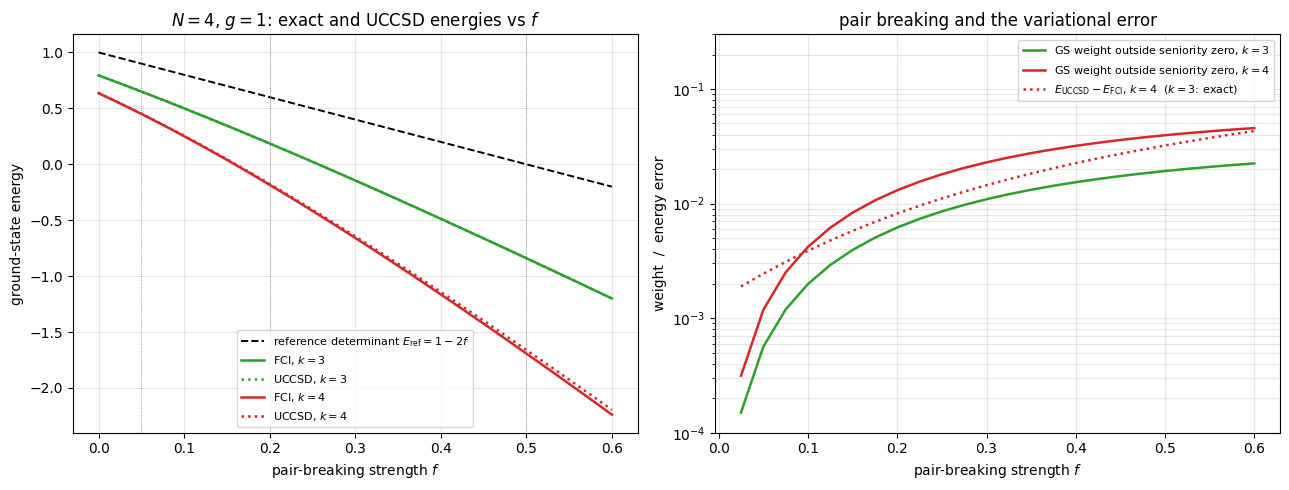
\includegraphics[width=\linewidth]{figs/fig12.png}
\caption{The pairing model with the particle-hole term, $N=4$, $g=1$, as a
function of the pair-breaking strength $f$.  Left: energy of the reference
determinant (dashed), exact ground-state energy (solid) and UCCSD energy
(dotted) at $k=3$ and $k=4$; the vertical lines mark the strengths
$f=0.05,0.2,0.5$ of Table~\ref{tab:ph}.  Right: weight of the exact ground
state outside the seniority-zero subspace (solid) and the UCCSD energy error at
$k=4$ (dotted; at $k=3$ the ansatz is exact).}
\label{fig:phscan}
\end{figure*}

\subsection{Refinement with pairs broken}
\label{sec:ph-refine}
We prolong the $k=2$ state --- at $N=4$ still a single determinant, now with
energy $E_{\rm low}=E_{\rm ref}$ --- into the $k=4$ space and evolve along the
path of Eq.~\eqref{eq:path} with the same shift rule $\mu=E_{\rm low}+0.6$, for
each $f$ (Fig.~\ref{fig:phrefine} and Table~\ref{tab:phrefine}).  Two things
change with $f$.  The target state acquires seniority-two components that the
prolonged determinant does not contain, and the effective pairing strength
$g+2f$ grows; both lower the initial overlap, from $0.868$ at $f=0$ to $0.600$
at $f=0.5$.  The minimum gap along the path, however, is still set by the shift,
$\Delta E_{\min}=0.600$ for every $f$ (the physical gap of $\Hhigh$ in fact
\emph{opens}, from $1.82$ to $2.86$), so the adiabatic time grows only because
the state has further to travel: $T^{*}$ rises from $16$ to $32$, and for every
$f$ the overlap exceeds $0.99$ with the energy converging to FCI from above.
The comparison with the coupling scan of Ref.~\cite{PairingCompanion} is
telling: there, the pure pairing model at $g=2$ --- the value of $g+2f$ at
$f=0.5$ --- had ${\rm ov}_0=0.617$ and $T^{*}=32$, almost exactly the numbers
found here at $f=0.5$.  The refinement cost of the seniority-breaking model is
thus governed by the renormalized pairing strength, and the genuinely new
$1p$--$1h$ and pair-breaking channels add only a small correction to it.
This is the same lesson as the coupling scan taught for the pairing force:
the practical limiter of the method is not a closing gap but a degrading
prolongation.  The $k=3\to4$ chain, started from the gate-level UCCSD state
whose singles now carry non-zero angles, buys the degradation back: it starts
at overlap $0.851$ even at $f=0.5$ and reaches $0.99$ at $T^{*}=26$ instead
of $32$.  Whether that saves gates is decided, as in
Ref.~\cite{PairingCompanion}, by the conditioned coarse term of
Eq.~\eqref{eq:Aterm}, which for the $3\to4$ chain is the complete $k=3$
Hamiltonian --- now $118$ Pauli strings instead of $34$
(Table~\ref{tab:pauli}) --- conditioned on the two appended qubits being
empty; we have not compiled it with the particle-hole term and quote the
$3\to4$ chain for its overlap only.

\begin{table}[t]
\caption{\label{tab:phrefine}Refinement to $k=4$ ($N=4$, $g=1$,
$\mu=E_{\rm low}+0.6$) with the particle-hole term: gap of $\Hhigh$, minimum
instantaneous gap along the path, initial overlap ${\rm ov}_0$ of the prolonged
state and adiabatic time $T^{*}$ to reach overlap $0.99$ (on the $T$ grid of
Sec.~\ref{sec:stages}; the $T^{*}=9$ quoted in Ref.~\cite{PairingCompanion}
for the $3\to4$ chain at $f=0$ used a finer grid), for the gate-free $2\to4$
chain and for the $3\to4$ chain started from the gate-level UCCSD state.}
\begin{ruledtabular}
\begin{tabular}{ccccccc}
& & & \multicolumn{2}{c}{$2\to4$} & \multicolumn{2}{c}{$3\to4$}\\
$f$ & gap($\Hhigh$) & $\Delta E_{\min}$ & ${\rm ov}_0$ & $T^{*}$ & ${\rm ov}_0$ & $T^{*}$\\
\colrule
0    & $1.823$ & $0.600$ & $0.868$ & $16$ & $0.964$ & $8$\\
0.05 & $1.943$ & $0.600$ & $0.841$ & $20$ & $0.955$ & $12$\\
0.2  & $2.289$ & $0.600$ & $0.751$ & $26$ & $0.921$ & $16$\\
0.5  & $2.860$ & $0.600$ & $0.600$ & $32$ & $0.851$ & $26$\\
\end{tabular}
\end{ruledtabular}
\end{table}

\begin{figure*}[t]
\centering
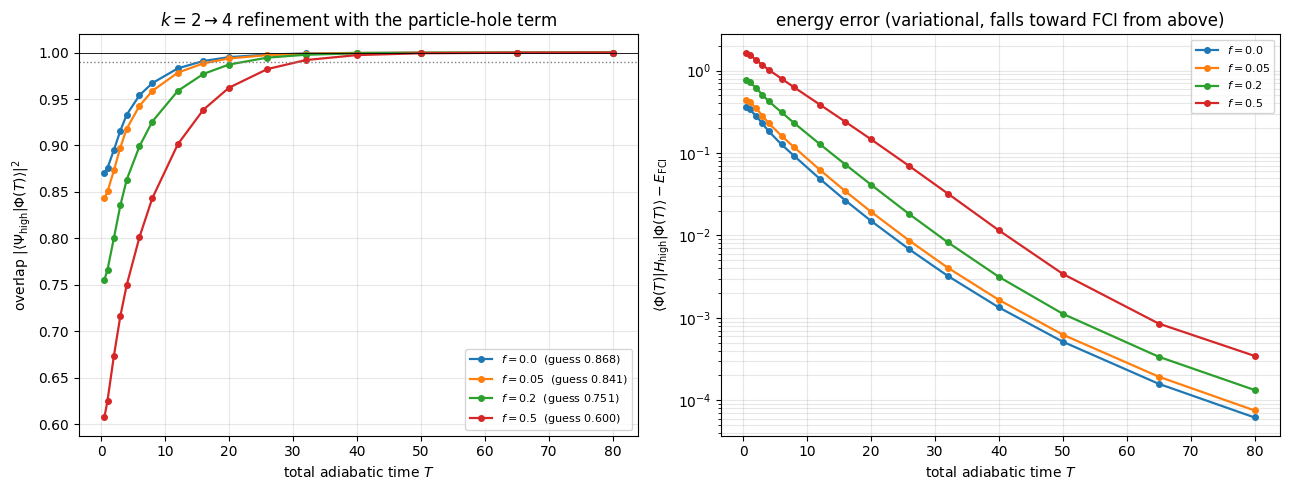
\includegraphics[width=\linewidth]{figs/fig13.png}
\caption{Resolution refinement $k=2\to4$ at $N=4$, $g=1$, for the pair-breaking
strengths $f=0,0.05,0.2,0.5$.  Left: overlap with the exact ground state versus
the adiabatic time $T$ (legend: initial overlap of the prolonged determinant;
dotted line: the $0.99$ target).  Right: variational energy error
$\expval{\Hhigh}{\Phi(T)}-E_{\rm FCI}$ on a logarithmic scale.}
\label{fig:phrefine}
\end{figure*}

\subsection{Sufficient conditions versus practice}
\label{sec:ph-bound}
The conditions of Eq.~\eqref{eq:Tbound} and the step condition that follows
it can be evaluated exactly for the path of Eq.~\eqref{eq:path}.  Writing
$A=P(\Hlow-\mu)P^\dagger$ and $B=\Hhigh-\mu$, the schedule gives
$\dot H=\tfrac{\pi}{2}\sin(\pi s)\,(B-A)$ and
$\ddot H=\tfrac{\pi^2}{2}\cos(\pi s)\,(B-A)$, so the integrand of
Eq.~\eqref{eq:Tbound} is fixed by the single number $\norm{B-A}$ and by the
instantaneous gap $\Delta(s)$, both taken in the $N=4$ sector in which the
evolution takes place.  Figure~\ref{fig:bound} shows the two along the
$k=2\to4$ path for the pure pairing force and the three particle-hole
strengths, and Table~\ref{tab:bound} collects the numbers; the $f=0$ row is
the reference of Sec.~\ref{sec:reference}.  Two opposite trends appear.  The
time bound hardly moves with $f$, $T_{\rm b}=4.3$--$5.1\times10^{3}$ for an
infidelity of $10^{-2}$: the minimum gap is set by the shift and is the same
$0.600$ for every $f$, the physical gap at $s=1$ opens, and $\norm{B-A}$
grows only from $7.62$ to $8.42$, so the integrand (which peaks near
$s\simeq0.25$, where $\sin(\pi s)$ is already sizable while the gap is
still close to its minimum, and is dominated by the term
$7\norm{\dot H}^2/\Delta^3$) integrates to $435$--$511$.  Since the empirical
$T^{*}$ doubles over the same range, the overshoot of the bound falls from
$3.2\times10^{2}$ at $f=0$ to $1.4\times10^{2}$ at $f=0.5$ --- the
particle-hole term brings practice closer to the bound, not by making the
bound tighter but by making the path genuinely longer.  The step condition
moves the other way.  The commutator sum $\Lambda_2$ over the Trotter groups
of the gate compilation (the conditioned coarse term, the diagonal term, the
six pair-hopping terms and, for $f\neq0$, the $48$ particle-hole blocks of
Sec.~\ref{sec:ph-cost}) grows from $13$ to $184$, and with it the first-order
step bound at $T^{*}$ from $3.4\times10^{4}$ to $1.9\times10^{6}$, while the
steps actually needed to reproduce the exact-slice overlap at $T^{*}$ to
within the adiabatic error of the path grow only from $160$ to $640$
(first order) and from $40$ to $160$ (second order).  The bound charges the
full norm of every new commutator, whereas the dynamics pays only for the
matrix elements that couple the tracked state to its neighbors, and the
small coefficient $f/2$ of the new blocks keeps the latter small.  The
ratios --- $1.4$--$3.2\times10^{2}$ for the time and $2\times10^{2}$ to
$3\times10^{3}$ for the step count --- are the fermionic, seniority-mixed
counterpart of what Ref.~\cite{Sadia2026} reports for nucleation of a
twelve-site Ising chain ($6\times10^{1}$ and $10^{7}$), and carry the same
message: the conditions certify convergence but do not predict cost.

\begin{figure*}[t]
\centering
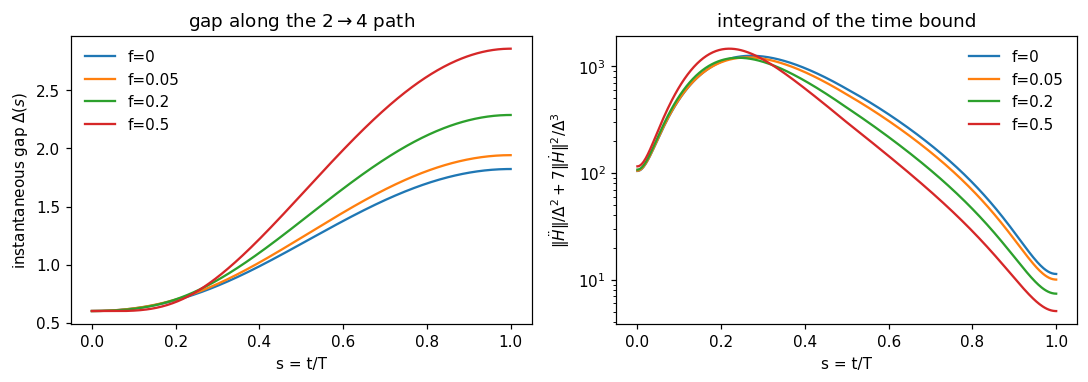
\includegraphics[width=\linewidth]{figs/fig18.png}
\caption{The ingredients of the adiabatic-time bound, Eq.~\eqref{eq:Tbound},
along the $k=2\to4$ refinement path at $N=4$, $g=1$, $\mu=E_{\rm low}+0.6$,
for the pure pairing model and the three particle-hole strengths.  Left:
instantaneous gap $\Delta(s)$ in the $N=4$ sector, from the shift-controlled
$0.600$ at $s=0$ to the physical gap of $\Hhigh$ at $s=1$, which opens with
$f$.  Right: the integrand
$\norm{\ddot H}/\Delta^2+7\norm{\dot H}^2/\Delta^3$ (logarithmic scale),
which peaks near $s\simeq0.25$ and integrates to $435$--$511$
(Table~\ref{tab:bound}).}
\label{fig:bound}
\end{figure*}

\begin{table*}[t]
\caption{\label{tab:bound}Sufficient conditions of Ref.~\cite{Sadia2026}
evaluated for the $k=2\to4$ refinement path ($N=4$, $g=1$,
$\mu=E_{\rm low}+0.6$; spectral norms in the $N=4$ sector) against the
empirical cost, for the pure pairing model ($f=0$, the reference of
Ref.~\cite{PairingCompanion}) and the three particle-hole strengths.
$\Delta_{\min}$: minimum instantaneous gap; $I$: the
integral in Eq.~\eqref{eq:Tbound}; $T_{\rm b}$: the time bound for infidelity
$\epsilon=10^{-2}$, $T_{\rm b}=I/\sqrt{\epsilon}$; $T^{*}$: time for overlap
$0.99$ (grid of Sec.~\ref{sec:stages}); $\Lambda_1=\max_s\norm{\dot H}$ and
$\Lambda_2=\max_s\sum_{i<j}\norm{[H_i,H_j]}$ over the Trotter groups of the
gate compilation; $n_{\rm b}(T^{*})$: first-order Trotter steps required by
the bound along the $T^{*}$ path at $\eta=\sqrt{\epsilon}/2$; $n_1$, $n_2$:
first- and second-order steps (from the sequence $5,10,20,\ldots$) that
reproduce the exact-slice overlap at $T^{*}$ to within the adiabatic error
$1-p(T^{*})$ of the path.}
\begin{ruledtabular}
\begin{tabular}{cccccccccccc}
$f$ & $\Delta_{\min}$ & $\norm{B-A}$ & $I$ & $T_{\rm b}$ & $T^{*}$ & $T_{\rm b}/T^{*}$ & $\Lambda_1$ & $\Lambda_2$ & $n_{\rm b}(T^{*})$ & $n_1$ & $n_2$\\
\colrule
0    & $0.600$ & $7.62$ & $511$ & $5.1\times10^{3}$ & $16$ & $3.2\times10^{2}$ & $12.0$ & $13.0$ & $3.4\times10^{4}$ & $160$ & $40$\\
0.05 & $0.600$ & $7.66$ & $480$ & $4.8\times10^{3}$ & $20$ & $2.4\times10^{2}$ & $12.0$ & $21.6$ & $8.8\times10^{4}$ & $320$ & $40$\\
0.2  & $0.600$ & $7.85$ & $435$ & $4.3\times10^{3}$ & $26$ & $1.7\times10^{2}$ & $12.3$ & $58.7$ & $4.0\times10^{5}$ & $320$ & $80$\\
0.5  & $0.600$ & $8.42$ & $446$ & $4.5\times10^{3}$ & $32$ & $1.4\times10^{2}$ & $13.2$ & $184$  & $1.9\times10^{6}$ & $640$ & $160$\\
\end{tabular}
\end{ruledtabular}
\end{table*}

\subsection{Rodeo filtering with a denser spectrum}
\label{sec:ph-rodeo}
The rodeo algorithm is the stage most exposed to the extra term, because its
energy scan sees the whole spectrum of the eight-qubit Hamiltonian in the $N=4$
sector, which the particle-hole term makes both denser and lower: $19$
eigenvalues lie below $E=4$ at $f=0.5$ against $14$ at $f=0$.
Figure~\ref{fig:phscanrodeo} shows the energy scan ($M=4$ cycles, $12$
time sets per energy) at the strongest coupling, $f=0.5$, feeding the filter
the resolution-refined ($T=25$) state with $p=0.980$ and, for contrast, the
prolonged determinant with $p=0.600$.  The coarse scan ($\sigma=2$) resolves
the ground state from the excited band --- helped by the larger gap --- and
the fine scan ($\sigma=8$) locates the peak at $E=-1.6924$ against the exact
$E_0=-1.691737$; with the refined input the excited-state structure that the
prolonged input shows above the $2^{-M}$ background is essentially gone.
Fixing $E=E_0$ and tracking the fidelity with the number of cycles for all
four strengths (Fig.~\ref{fig:phconv}; exact controlled evolution,
$\sigma=3$, $40$ Gaussian time sets), the infidelity falls geometrically
along the $\tfrac{1-p}{p}2^{-M}$ reference of Eq.~\eqref{eq:fid} and the
acceptance settles at the input overlap: after ten cycles
$1-\mathcal{F}=2.0\times10^{-6}$, $2.9\times10^{-6}$, $4.6\times10^{-6}$ and
$4.5\times10^{-5}$ for $f=0$, $0.05$, $0.2$ and $0.5$, with acceptances
$0.998$, $0.997$, $0.994$ and $0.980$.  The pair-breaking channels cost the
pipeline one order of magnitude in final infidelity at the strongest coupling
--- recoverable with three more cycles --- and nothing in acceptance beyond the
lower input overlap.  The denser spectrum does not slow the filter: the
physical gap opens with $f$ (Table~\ref{tab:phrefine}), so the smallest
excitation energy carrying weight satisfies $\Delta_{\min}\sigma\ge5$ at
$\sigma=3$ and the single-cycle suppression factor of Eq.~\eqref{eq:fid}
stays close to $1/2$.

\begin{figure*}[t]
\centering
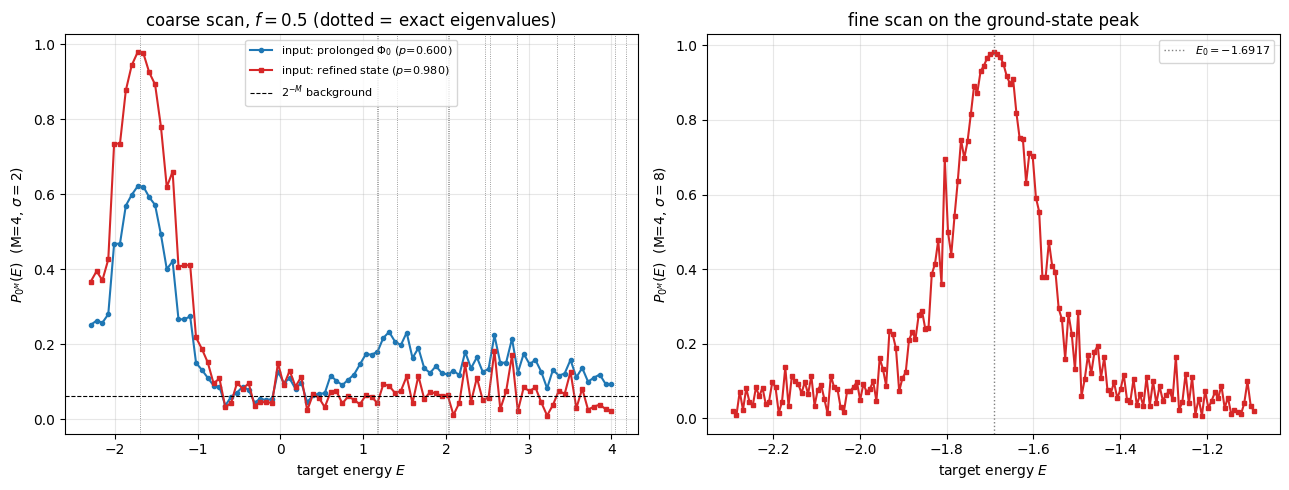
\includegraphics[width=\linewidth]{figs/fig14.png}
\caption{Rodeo energy scan ($M=4$) for the pairing model with the particle-hole
term at $f=0.5$.  Left: coarse scan ($\sigma=2$) from the prolonged determinant
($p=0.600$) and from the resolution-refined state ($p=0.980$); dotted vertical
lines mark the exact eigenvalues, the dashed line the $2^{-M}$ background.
Right: fine scan ($\sigma=8$) on the ground-state peak, located at $E=-1.6924$
(exact $E_0=-1.6917$).}
\label{fig:phscanrodeo}
\end{figure*}

\begin{figure*}[t]
\centering
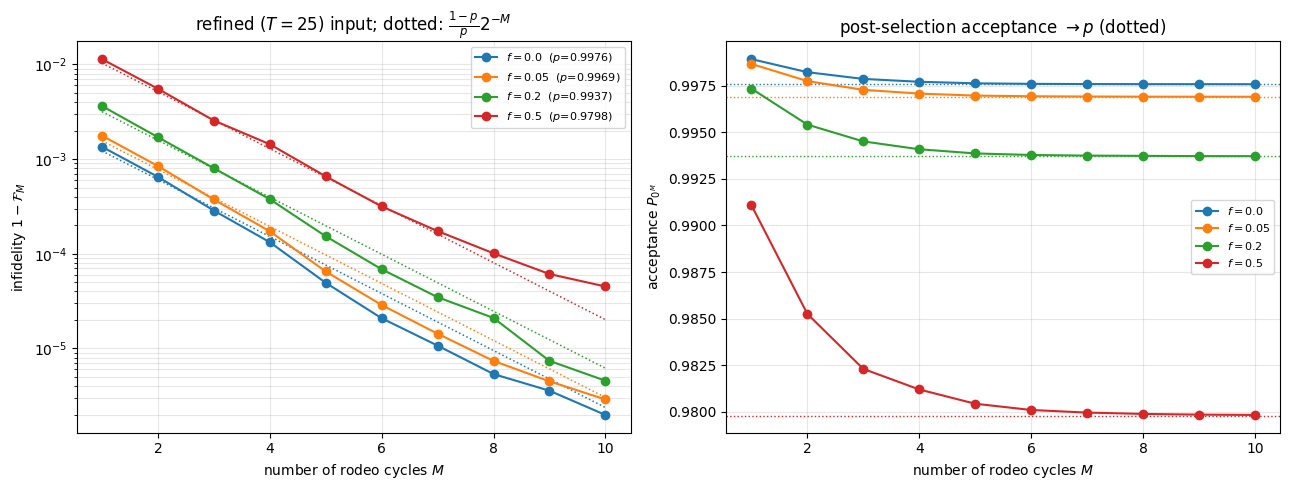
\includegraphics[width=\linewidth]{figs/fig15.png}
\caption{Rodeo eigenstate preparation at $E=E_0$ with the particle-hole term,
for $f=0,0.05,0.2,0.5$, from the resolution-refined ($T=25$) input, averaged
over $40$ random time sets ($\sigma=3$).  Left: post-selected infidelity versus
the number of cycles $M$ (dotted: $\tfrac{1-p}{p}2^{-M}$).  Right: the
acceptance converges to the input overlap $p$ (dotted).}
\label{fig:phconv}
\end{figure*}

% ===========================================================================
\section{The circuit-level budget with the particle-hole term}
\label{sec:circuits}
% ===========================================================================
\label{sec:ph-cost}
The pipeline itself is unchanged by $\Vph$ --- prolongation, the adiabatic
path, the shift rule and the rodeo cycle were all written for the $2k$-qubit
register --- but the Hamiltonian that is Trotterized is not
(Table~\ref{tab:pauli}).  To extend the circuit-level analysis of
Ref.~\cite{PairingCompanion} we decompose $\Vph$ into exactly exponentiable
blocks in the same spirit as the pair-hopping terms.  Its $q=r$ pieces are
pairing terms and only rescale the rotation angles of the existing blocks
($g\to g+2f$), at no cost.  The remaining pieces, one per $(p,q,r)$ with
$q\neq r$, fall into two families: $2k(k-1)$ one-particle--one-hole blocks
($a^\dagger_{p\uparrow}n_{p\downarrow}a_{r\uparrow}+{\rm h.c.}$ and the
spin-flipped partner), each a sum of four Pauli strings, and $k(k-1)(k-2)$
pair-breaking blocks (eight strings each, like a double excitation).  Within
each block the strings mutually commute, so every factor $e^{-i\hat T\delta t}$
is realized exactly by its rotations and the product-formula error again comes
only from the non-commutativity \emph{between} blocks: $55$ of them at $k=4$
instead of seven.

Two things follow, both quantified in Fig.~\ref{fig:phtrotter} and
Table~\ref{tab:phdepth}.  First, the Trotter error at fixed step count grows
only modestly --- at $t=1$, $k=4$ the second-order error with sixteen steps is
$2.1\times10^{-3}$, $3.8\times10^{-3}$ and $7.5\times10^{-3}$ for $f=0$,
$0.2$, $0.5$ --- because the new blocks carry the small coefficient $f/2$.
The Trotterized refinement reaches its exact-slice value with the same
$n_s=80$ second-order steps at $f=0.2$ (overlap $0.9961$ against $0.9969$),
and the rodeo cycle at $\delta t=0.25$ keeps an acceptance of $0.96$ with an
infidelity of $3.8\times10^{-4}$ after six cycles, essentially the
pairing-model operating point.  At $f=0.5$ the step $\delta t=0.25$ begins to
fail --- acceptance $0.84$, the symptom of a corrupted evolution recalled in
Sec.~\ref{sec:reference} --- and $\delta t=0.125$ restores it to $0.97$ with
an infidelity of $6\times10^{-4}$ against $5\times10^{-4}$ for exact
evolution.  The filter is thus again diagnostic of its own Trotter error,
and the diagnostic is reached at a step size that was safe for the pairing
force; since the number and structure of the Trotter blocks are the same at
$f=0.2$ and $f=0.5$, it is the strength of the new channels, not their
number, that shrinks the admissible step.  Second, the depth of one step
grows ninefold: compiled block by block with the ladder rule of
Eq.~\eqref{eq:trottercost}, a first-order step costs $2728$ CNOTs instead of
$296$ ($348$ rotations instead of $60$; $3424$ against $416$ once
controlled), the $1p$--$1h$ family contributing $640$ and the pair-breaking
family $1792$ CNOTs; the coarse term is unchanged ($14$ CNOTs, the coarse
space is still one determinant).  The budget per accepted preparation
therefore scales almost exactly with the step cost: at the pairing-model
operating point ($n_s=80$, $M=2$, $\delta t=0.25$) it is $6.5\times10^{5}$
CNOTs at $f=0.2$ against $7.2\times10^{4}$ for the pure pairing force, for an
infidelity of $1.0\times10^{-3}$, and at $f=0.5$ the finer rodeo step brings
the total to $8.3\times10^{5}$ CNOTs for $5.3\times10^{-3}$.  The price of a
more realistic interaction thus appears where it should, in the depth of
each Trotter step of the Hamiltonian evolution, and not in the structure,
the operating point or the convergence of the pipeline.

Measured against the right comparator, however, the extra depth buys no
accuracy advantage.  The actual infidelity of the UCCSD state is
$1.0\times10^{-3}$ at $f=0.2$ and $3.7\times10^{-3}$ at $f=0.5$
(Table~\ref{tab:ph}), so the hybrid at $M=2$ is tied with the
\emph{unfiltered} variational state at $f=0.2$ and behind it at $f=0.5$; and
the same filter applied to the UCCSD input (last column of
Table~\ref{tab:phdepth}) reaches $5.1\times10^{-4}$ and $2.0\times10^{-3}$ at
$\delta t=0.25$, $2.6\times10^{-4}$ and $9.6\times10^{-4}$ at $\delta t=0.125$,
for $2.0$--$3.8\times10^{5}$ CNOTs per accepted preparation --- a factor two to
three below the hybrid in cost and two to five below it in infidelity.  The
reason is the one identified in Sec.~\ref{sec:ph-refine}: the variational
input degrades with $f$, but so does the prolonged starting state of the
refinement, from $p=0.868$ to $0.600$, so the refinement must travel further
--- $T^{*}$ doubles --- along a path whose every step has become nine times
deeper.  The
seniority-breaking term thus confirms the structural robustness of the
pipeline and, at the same time, the negative conclusion of
Ref.~\cite{PairingCompanion}.

\begin{figure*}[t]
\centering
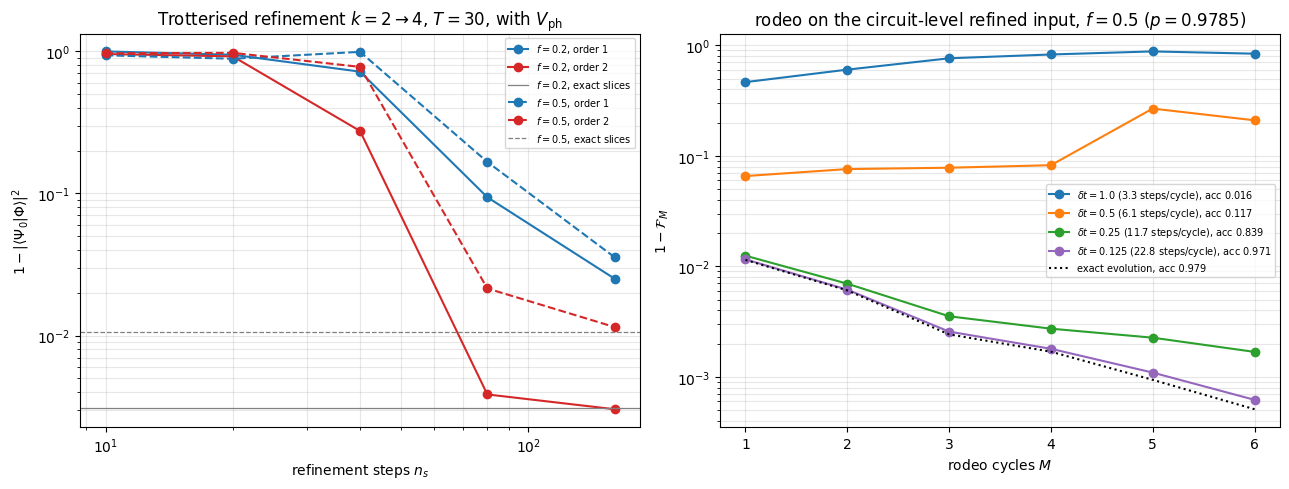
\includegraphics[width=\linewidth]{figs/fig16.png}
\caption{The pipeline at the circuit level with the particle-hole term
($k=4$, $N=4$, $g=1$).  Left: infidelity of the Trotterized refinement
$k=2\to4$ ($T=30$) versus the number of product-formula steps $n_s$ for
first- and second-order formulas at $f=0.2$ (solid) and $f=0.5$ (dashed);
horizontal lines mark the exact-slice refinement.  Right: rodeo infidelity
versus cycles at $f=0.5$ on the circuit-level refined input ($n_s=80$,
second order, $p=0.9785$) with the controlled evolution Trotterized at fixed
step sizes $\delta t$; the legend gives the mean number of steps per cycle and
the six-cycle acceptance.}
\label{fig:phtrotter}
\end{figure*}

\begin{table*}[t]
\caption{\label{tab:phdepth}Gate budget at $k=4$ ($N=4$, $g=1$) with the
particle-hole term, per accepted preparation, at the operating point of
Sec.~\ref{sec:cost} ($n_s=80$ second-order refinement steps at $T=30$, $M=2$
rodeo cycles, $\sigma=4$) for two rodeo step sizes $\delta t$.  Step costs are
the block-by-block CNOT counts (uncontrolled / controlled); the refinement
column includes the $14$-CNOT coarse term per half-step; the rodeo column uses
the mean number of Trotter steps over the two cycles, doubled for the symmetric
formula.  The last two columns give the infidelity of the hybrid and, for
comparison, the infidelity of the unfiltered UCCSD state ($1\,312$ CNOTs,
$26$ parameters, the same circuit for every $f$) and of the UCCSD state passed
through the same two-cycle filter, with its CNOTs per accepted preparation in
parentheses.  The first row is the pure pairing model of
Ref.~\cite{PairingCompanion}.}
\footnotesize
\begin{ruledtabular}
\begin{tabular}{cccccccc cc}
$f$ & $\delta t$ & step (unctrl./ctrl.) & refinement & rodeo & per run & $P_M$ & per accepted & $1-\mathcal{F}$: hybrid / UCCSD & UCCSD$+$rodeo (CNOTs)\\
\colrule
$0$   & $0.25$  & $296$ / $416$   & $49\,600$  & $22\,000$ & $71\,600$ & $0.994$ & $7.2\times10^{4}$ & $5.3\times10^{-4}$ / $1.8\times10^{-4}$ & $1.3\times10^{-4}$ ($2.3\times10^{4}$)\\
$0.2$ & $0.25$  & $2728$ / $3424$ & $438\,720$ & $190\,603$ & $629\,323$ & $0.972$ & $6.5\times10^{5}$ & $1.0\times10^{-3}$ / $1.0\times10^{-3}$ & $5.1\times10^{-4}$ ($2.0\times10^{5}$)\\
$0.2$ & $0.125$ & $2728$ / $3424$ & $438\,720$ & $375\,499$ & $814\,219$ & $0.996$ & $8.2\times10^{5}$ & $8.1\times10^{-4}$ / $1.0\times10^{-3}$ & $2.6\times10^{-4}$ ($3.8\times10^{5}$)\\
$0.5$ & $0.25$  & $2728$ / $3424$ & $438\,720$ & $190\,603$ & $629\,323$ & $0.891$ & $7.1\times10^{5}$ & $6.1\times10^{-3}$ / $3.7\times10^{-3}$ & $2.0\times10^{-3}$ ($2.1\times10^{5}$)\\
$0.5$ & $0.125$ & $2728$ / $3424$ & $438\,720$ & $375\,499$ & $814\,219$ & $0.979$ & $8.3\times10^{5}$ & $5.3\times10^{-3}$ / $3.7\times10^{-3}$ & $9.6\times10^{-4}$ ($3.8\times10^{5}$)\\
\end{tabular}
\end{ruledtabular}
\end{table*}

% ===========================================================================
\section{Discussion and outlook}
\label{sec:discussion}
% ===========================================================================
Opening the particle-hole channel changes the Hamiltonian in exactly the
ways that make the pure pairing model a special case --- the seniority is
mixed, the spectrum is denser, the reference determinant is no longer
self-consistent, singles switch on in the variational ansatz, and the
compact pair-to-qubit encoding is gone --- and leaves the pipeline
untouched.  The same prolongation, the same shift rule, the same adiabatic
path and the same filter run on the eight-qubit register without any
modification, the path gap stays at the shift-controlled $0.600$ for every
strength, the refinement time doubles for the same reason it grew in the
coupling scan of the pairing force --- a poorer prolonged start, governed
here by the renormalized strength $g+2f$ --- and the rodeo filter converges
geometrically to $10^{-5}$--$10^{-6}$ in ten cycles with the acceptance at
the input overlap.  The sufficient conditions of Ref.~\cite{Sadia2026} are
consistent with this picture from the other side: the time bound is
insensitive to the pair breaking because the minimum gap is set by the
shift, while the step bound, which charges the full norm of every new
commutator, grows by almost two orders of magnitude where practice grows by a
factor four.  Everything the particle-hole term costs is in the depth of a
Trotter step, $296\to2728$ CNOTs, traceable string by string to
Table~\ref{tab:pauli}, and the budget per accepted preparation scales with
it, from $7\times10^{4}$ to $6$--$8\times10^{5}$ CNOTs.

The question that motivated the extension --- whether the refinement stage
begins to earn its gates once the single-reference variational input starts
to fail --- receives, at these strengths, a negative answer, and the reason
is instructive.  The UCCSD infidelity does degrade twentyfold across the
scan, from $1.8\times10^{-4}$ to $3.7\times10^{-3}$, as the exact ground
state acquires up to $3.9\%$ seniority-two weight that a fixed
single-reference ansatz from an unrelaxed determinant captures imperfectly.
But the prolonged starting state of the refinement, which is the same
determinant, degrades as well --- from $p=0.868$ to $0.600$, with $T^{*}$
doubling --- so the adiabatic stage has further to travel along a path whose
every step has become nine times deeper, and at the operating point the
hybrid is tied with the unfiltered UCCSD state at $f=0.2$, behind it at
$f=0.5$, and behind the filtered UCCSD state by a factor two to three in
cost and two to five in infidelity at both strengths compiled
(Table~\ref{tab:phdepth}).
  A regime in which refinement wins
must therefore combine a poor full-space variational input with a good
coarse one, so that the prolonged overlap stays high while the fine-space
ansatz fails; the $3\to4$ chain, which starts at overlap $0.851$ even at
$f=0.5$, is the natural candidate, but it carries the conditioned $k=3$
Hamiltonian --- now $118$ Pauli strings --- along the whole path, and in
Ref.~\cite{PairingCompanion} that coarse term already cost more per
application than the fine-space step itself.  Whether the balance tips with
the particle-hole term is a compilation we have not carried out, and we list
it below.  Two further caveats apply to the comparator.  The reference
determinant was not re-optimized, so part of what the singles absorb is
mean-field relaxation; a Hartree--Fock-optimized reference would lower the
variational error at $f\neq0$ and, by the same token, raise the prolonged
overlap of a refinement started from it, so the comparison is between two
unrelaxed starts and should be repeated with relaxed ones.  And the
variational numbers are those of one optimizer from one start, which
document the accuracy of this preparation rather than the expressivity of
the ansatz.

\paragraph{Encodings and the pairing-model literature.}
The seniority-breaking term is also the point at which the present work and
the pairing-model programme of Lacroix and collaborators part company at the
level of the register.  The symmetry-restoration
route~\cite{Lacroix2020,RuizGuzman2022,RuizGuzman2023,RuizGuzman2024,Lacroix2023EPJA},
the ADAPT-VQE studies~\cite{Zhang2024,Zhang2025} and the Green's-function
construction of Ref.~\cite{AychetClaisse2026} are formulated for the
seniority-conserving pairing force, for which one qubit per level suffices
and the $N=4$, $k=4$ problem is a six-dimensional block; with $\Vph$ that
block becomes the $36$-dimensional $S_z=0$ sector of a fermionic register,
and every gate count of Sec.~\ref{sec:circuits} refers to the $2k$-qubit
Jordan--Wigner encoding on which it is written.  The structural relation
between the two approaches is unchanged by the term: both start from a
cheap, imperfect trial state and sharpen it, the symmetry-restoration route
by projecting on a symmetry quantum number and ours by filtering in energy
along a gapped path across resolutions, the two filters being the same
resource --- one ancilla, a controlled unitary and a post-selected
measurement --- that compose.  What the particle-hole term adds is the
observation of Ref.~\cite{Zhang2024} seen from the other side: there,
ADAPT-VQE with a symmetry-breaking pool could collapse to unphysical
energies on degenerate pairing systems, and a downstream energy filter
cannot repair an input of zero overlap or separate degenerate states by
energy alone; here, the Hamiltonian itself breaks the seniority, the
singles and pair-breaking doubles of a symmetry-conserving pool are
physical, and the filter has nothing to repair but the adiabatic tail.  A
seniority-mixed Hamiltonian is, in that sense, the natural target for an
ADAPT-style input with a full singles-and-doubles pool, and its inclusion as
a comparator is the obvious next step.

\paragraph{Hardware requirements.}
The Trotterized pipeline quantifies the dominant coherent error of an ideal
device, and the requirements with the particle-hole term are explicit:
$2k+1=9$ qubits at $k=4$; a mid-circuit measurement with reset and reuse of
one ancilla; arbitrary-angle $R_z$ rotations, $160$ per UCCSD preparation
and $348$ per Trotter step (against $60$ for the pairing force); and a
coherent budget per accepted preparation of $2$--$4\times10^{5}$ two-qubit
gates for the cheapest route of Table~\ref{tab:phdepth} (UCCSD input, two
cycles) and $6$--$8\times10^{5}$ for the refined input, on top of the energy
scan and the repetitions needed to estimate acceptance probabilities.  At
the two-qubit error rates demonstrated in large-scale experiments today ---
of order $10^{-2}$ on the superconducting processor of Ref.~\cite{Kim2023}
and $(0.8$--$2)\times10^{-3}$ on trapped-ion
processors~\cite{Moses2023,Ransford2025} --- a $10^{5}$-gate run suffers of
order one hundred faults even on the best of these, and the full
particle-hole budget is nearly an order of magnitude beyond that; none of it is
executable with physical qubits without substantial error mitigation, and
it is a workload for the first generation of logical-qubit machines, such as
the neutral-atom systems on which logical circuits with mid-circuit readout
have been demonstrated~\cite{Bluvstein2024,Reichardt2024} and the machine
planned by the QuNorth initiative~\cite{QuNorth}; Table~\ref{tab:phdepth} is
offered as its specification.  Connectivity matters more than for the
pairing force: all-to-all connectivity absorbs the Jordan--Wigner ladders
without SWAP overhead, and on square or heavy-hex lattices the weight-$4$
pair-hopping rotations act on adjacent qubits, but the weight-$2k$ strings
of the $1p$--$1h$ family do not, so routing costs are no longer bounded by
the pair structure.  A proportionate near-term target remains a mitigated
$k=3$ demonstration on seven qubits, where the Hamiltonian has $118$ strings
of weight up to six, with a short refinement schedule and one or two rodeo
cycles, and where the collapse of the acceptance under a corrupted evolution
--- reached here already at $\delta t=0.25$, $f=0.5$ --- doubles as a hardware
diagnostic.

\paragraph{Concluding remarks and perspectives.}
The pairing model with a particle-hole interaction is the smallest
Hamiltonian that has the central ingredients of a realistic two-body
interaction --- pair scattering, one-particle--one-hole excitations and pair
breaking --- while remaining exactly solvable in a $70$-dimensional sector
against which every stage of a quantum state-preparation pipeline can be
validated, and the present results establish how resolution refinement
followed by the rodeo algorithm behaves on it: unchanged in structure and
convergence, nine times deeper per Trotter step, and still not a gate saving
over filtering a cheap variational input, which the term degrades but does
not break.  Four extensions follow directly.  First, the comparators that
the seniority-mixed Hamiltonian calls for: a Hartree--Fock-relaxed
reference for both the variational ansatz and the prolonged start, an
ADAPT-VQE input with a full singles-and-doubles pool, and the compiled
$3\to4$ chain with the conditioned $k=3$ particle-hole Hamiltonian, which is
where a regime favorable to refinement would first appear.  Second, an
optimized refinement in the sense of the optimized nucleation of
Ref.~\cite{Sadia2026} --- the Trotterized path of Eq.~\eqref{eq:path} as a
warm-started variational circuit with a few layers per stage --- for which
the ninefold step depth of the particle-hole model is precisely the
motivation.  Third, other seniority-breaking Hamiltonians on which the same
refinement-plus-filter analysis can be repeated against exact
diagonalization, the Hubbard model on small lattices being the obvious next
case, since there basis refinement and the lattice growth of nucleation can
be composed with the same Trotterized machinery.  Fourth, a mitigated
seven-qubit demonstration on present devices, followed by the nine-qubit
budget of Table~\ref{tab:phdepth} on an early logical-qubit machine.

% ===========================================================================
\section*{Code availability}
The complete implementation --- pairing Hamiltonian with and without the
particle-hole term, gate-level UCCSD--VQE, prolongation, adiabatic refinement,
and the ancilla-based rodeo algorithm --- is provided as a tested Python package
and a single Jupyter notebook, shared with Ref.~\cite{PairingCompanion}, that
reproduces every figure and number in this article.
Give GitHub link when everything is ready.
\begin{acknowledgments}
The work of C.G. and G.F.L. acknowledge funding from the
European Union’s Horizon Europe research and innovation program under the Marie Skłodowska-Curie Grant Agreement No.
101126636. M.H.-J. is partially supported by U.S. National Science Foundation
(NSF) Grants PHY-1404159 and PHY-2310020.
The authors  acknowledge Anthropic’s Claude
for assistance with literature search and coding.

\end{acknowledgments}

% ===========================================================================
\begin{thebibliography}{99}
% ===========================================================================
\bibitem{PairingCompanion}
S.~Bogner, C.~Glittum, H.~Hergert, M.~Hjorth-Jensen, G.~Lange, R.~LaRose,
D.~Lee, F.~P.~Massel, J.~P.~Sadia,
\textit{Resolution refinement followed by the rodeo algorithm for eigenstate
preparation: implementation and assessment on the pairing Hamiltonian},
companion paper (2026).

\bibitem{Beck2023}
D.~Beck \textit{et al.},
\textit{Quantum information science and technology for nuclear physics.
Input into U.S.\ long-range planning, 2023},
arXiv:2303.00113 (2023).

\bibitem{Bauer2023}
C.~W.~Bauer, Z.~Davoudi, N.~Klco, M.~J.~Savage,
\textit{Quantum simulation of fundamental particles and forces},
Nat.\ Rev.\ Phys.\ \textbf{5}, 420 (2023).

\bibitem{LeeReview2023}
D.~Lee,
\textit{Quantum techniques for eigenvalue problems},
Eur.\ Phys.\ J.\ A \textbf{59}, 275 (2023).

\bibitem{Ovrum2007}
E.~Ovrum, M.~Hjorth-Jensen,
\textit{Quantum computation algorithm for many-body studies},
arXiv:0705.1928 (2007).

\bibitem{Hlatshwayo2022}
M.~Q.~Hlatshwayo, Y.~Zhang, H.~Wibowo, R.~LaRose, D.~Lacroix, E.~Litvinova,
\textit{Simulating excited states of the Lipkin model on a quantum computer},
Phys.\ Rev.\ C \textbf{106}, 024319 (2022).

\bibitem{Stetcu2022}
I.~Stetcu, A.~Baroni, J.~Carlson,
\textit{Variational approaches to constructing the many-body nuclear ground state
for quantum computing},
Phys.\ Rev.\ C \textbf{105}, 064308 (2022).

\bibitem{PerezObiol2023}
A.~P\'erez-Obiol, A.~M.~Romero, J.~Men\'endez, A.~Rios, A.~Garc\'ia-S\'aez,
B.~Juli\'a-D\'iaz,
\textit{Nuclear shell-model simulation in digital quantum computers},
Sci.\ Rep.\ \textbf{13}, 12291 (2023).

\bibitem{Jiang2023}
C.~Jiang, J.~Pei,
\textit{Quantum computing of the pairing Hamiltonian at finite temperature},
Phys.\ Rev.\ C \textbf{107}, 044308 (2023).

\bibitem{Zhang2024}
J.~Zhang, D.~Lacroix, Y.~Beaujeault-Taudi\`ere,
\textit{Neutron-proton pairing correlations described on quantum computers},
Phys.\ Rev.\ C \textbf{110}, 064320 (2024).

\bibitem{Lacroix2023}
E.~A.~Ruiz~Guzman,
\textit{Symmetry breaking and restoration for many-body problems treated on
quantum computers},
PhD thesis, Universit\'e Paris-Saclay (2023); arXiv:2310.17996.

\bibitem{Richardson1963}
R.~W.~Richardson,
\textit{A restricted class of exact eigenstates of the pairing-force Hamiltonian},
Phys.\ Lett.\ \textbf{3}, 277 (1963).

\bibitem{RichardsonSherman1964}
R.~W.~Richardson, N.~Sherman,
\textit{Exact eigenstates of the pairing-force Hamiltonian},
Nucl.\ Phys.\ \textbf{52}, 221 (1964).

\bibitem{Dukelsky2004}
J.~Dukelsky, S.~Pittel, G.~Sierra,
\textit{Colloquium: Exactly solvable Richardson-Gaudin models for many-body
quantum systems},
Rev.\ Mod.\ Phys.\ \textbf{76}, 643 (2004).

\bibitem{Lacroix2020}
D.~Lacroix,
\textit{Symmetry assisted preparation of entangled many-body states on a quantum computer},
Phys.\ Rev.\ Lett.\ \textbf{125}, 230502 (2020).

\bibitem{RuizGuzman2022}
E.~A.~Ruiz~Guzman, D.~Lacroix,
\textit{Accessing ground-state and excited-state energies in a many-body system after symmetry restoration using quantum computers},
Phys.\ Rev.\ C \textbf{105}, 024324 (2022).

\bibitem{RuizGuzman2023}
E.~A.~Ruiz~Guzman, D.~Lacroix,
\textit{Restoring broken symmetries using quantum search ``oracles''},
Phys.\ Rev.\ C \textbf{107}, 034310 (2023).

\bibitem{RuizGuzman2024}
E.~A.~Ruiz~Guzman, D.~Lacroix,
\textit{Restoring symmetries in quantum computing using Classical Shadows},
Eur.\ Phys.\ J.\ A \textbf{60}, 112 (2024).

\bibitem{Lacroix2023EPJA}
D.~Lacroix, E.~A.~Ruiz~Guzman, P.~Siwach,
\textit{Symmetry breaking/symmetry preserving circuits and symmetry restoration on quantum computers: A quantum many-body perspective},
Eur.\ Phys.\ J.\ A \textbf{59}, 3 (2023).

\bibitem{Ayral2023}
T.~Ayral, P.~Besserve, D.~Lacroix, E.~A.~Ruiz~Guzman,
\textit{Quantum computing with and for many-body physics},
Eur.\ Phys.\ J.\ A \textbf{59}, 227 (2023).

\bibitem{Zhang2025}
J.~Zhang, D.~Lacroix,
\textit{Excited states from ADAPT-VQE convergence path in many-body problems: application to nuclear pairing problem and H$_4$ molecule dissociation},
Phys.\ Lett.\ B \textbf{869}, 139841 (2025).

\bibitem{AychetClaisse2026}
S.~Aychet-Claisse, D.~Lacroix, V.~Som\`a, J.~Zhang,
\textit{Quantum simulations of Green's functions for small superfluid systems},
Phys.\ Rev.\ C \textbf{113}, 044324 (2026); arXiv:2509.02272.

\bibitem{Bogner2026}
S.~Bogner, H.~Hergert, M.~Hjorth-Jensen, R.~LaRose, D.~Lee, M.~Patkowski,
\textit{Quantum state preparation with resolution refinement},
Phys.\ Lett.\ B \textbf{875}, 140363 (2026); arXiv:2511.14732.

\bibitem{Choi2021}
K.~Choi, D.~Lee, J.~Bonitati, Z.~Qian, J.~Watkins,
\textit{Rodeo algorithm for quantum computing},
Phys.\ Rev.\ Lett.\ \textbf{127}, 040505 (2021).

\bibitem{Qian2024}
Z.~Qian, J.~Watkins, G.~Given, J.~Bonitati, K.~Choi, D.~Lee,
\textit{Demonstration of the rodeo algorithm on a quantum computer},
Eur.\ Phys.\ J.\ A \textbf{60}, 151 (2024).

\bibitem{Hirsch2002}
J.~G.~Hirsch, A.~Mariano, J.~Dukelsky, P.~Schuck,
\textit{Fully self-consistent RPA description of the many level pairing model},
Ann.\ Phys.\ (N.Y.) \textbf{296}, 187 (2002).

\bibitem{Dang2006}
N.~Dinh~Dang,
\textit{Consistency of particle-particle random-phase approximation and its
renormalizations},
Phys.\ Rev.\ C \textbf{74}, 034326 (2006).

\bibitem{RingSchuck}
P.~Ring, P.~Schuck,
\textit{The Nuclear Many-Body Problem},
Springer, Berlin (1980).

\bibitem{MHJbook}
M.~Hjorth-Jensen,
\textit{Quantum Mechanics for Many-Particle Systems},
lecture notes, University of Oslo (2026), Chapter~4.

\bibitem{LeeUCC2019}
J.~Lee, W.~J.~Huggins, M.~Head-Gordon, K.~B.~Whaley,
\textit{Generalized unitary coupled cluster wavefunctions for quantum computation},
J.\ Chem.\ Theory Comput.\ \textbf{15}, 311 (2019).

\bibitem{Tilly2022}
J.~Tilly, H.~Chen, S.~Cao, D.~Picozzi, K.~Setia, Y.~Li, E.~Grant, L.~Wossnig,
I.~Rungger, G.~H.~Booth, J.~Tennyson,
\textit{The variational quantum eigensolver: a review of methods and best
practices},
Phys.\ Rep.\ \textbf{986}, 1 (2022).

\bibitem{NielsenChuang}
M.~A.~Nielsen, I.~L.~Chuang,
\textit{Quantum Computation and Quantum Information},
Cambridge University Press (2010).

\bibitem{Jansen2007}
S.~Jansen, M.-B.~Ruskai, R.~Seiler,
\textit{Bounds for the adiabatic approximation with applications to quantum
computation},
J.\ Math.\ Phys.\ \textbf{48}, 102111 (2007).

\bibitem{Sadia2026}
J.~P.~Sadia, M.~Hjorth-Jensen, D.~Lee, R.~LaRose,
\textit{Digital quantum state preparation by nucleation},
arXiv:2609.37527 (2026).

\bibitem{Kovalsky2023}
L.~K.~Kovalsky, F.~A.~Calderon-Vargas, M.~D.~Grace, A.~B.~Magann,
J.~B.~Larsen, A.~D.~Baczewski, M.~Sarovar,
\textit{Self-healing of Trotter error in digital adiabatic state preparation},
Phys.\ Rev.\ Lett.\ \textbf{131}, 060602 (2023).

\bibitem{Kim2023}
Y.~Kim, A.~Eddins, S.~Anand, K.~X.~Wei, E.~van~den~Berg, S.~Rosenblatt,
H.~Nayfeh, Y.~Wu, M.~Zaletel, K.~Temme, A.~Kandala,
\textit{Evidence for the utility of quantum computing before fault tolerance},
Nature \textbf{618}, 500 (2023).

\bibitem{Moses2023}
S.~A.~Moses \textit{et al.},
\textit{A race-track trapped-ion quantum processor},
Phys.\ Rev.\ X \textbf{13}, 041052 (2023).

\bibitem{Ransford2025}
A.~Ransford \textit{et al.},
\textit{Helios: a 98-qubit trapped-ion quantum computer},
arXiv:2511.05465 (2025).

\bibitem{Bluvstein2024}
D.~Bluvstein \textit{et al.},
\textit{Logical quantum processor based on reconfigurable atom arrays},
Nature \textbf{626}, 58 (2024).

\bibitem{Reichardt2024}
B.~W.~Reichardt \textit{et al.},
\textit{Logical computation demonstrated with a neutral atom quantum processor},
arXiv:2411.11822 (2024).

\bibitem{QuNorth}
QuNorth, \textit{Magne: a level-2 neutral-atom quantum computer},
\url{https://qunorth.com} (accessed July 2026).
\end{thebibliography}

\end{document}
